% ! TeX root = ../../master-thesis.tex

\chapter{Implementation}
\label{chapter:implementation}

This chapter describes the concrete solution implemented for this project,
building upon the design presented in the previous chapter. First, it
introduces the implementations of several simulators, including a general
simulator (Section \ref{section:implementation:simulator}), a step-by-step
simulator (Section \ref{section:implementation:step-simulator}), a concurrent
simulator (Section \ref{section:implementation:concurrent-simulator}), and a
convergence simulator (Section
\ref{section:implementation:convergence-simulator}). Then, Sections
\ref{section:implementation:stream-extension} and
\ref{section:implementation:finite-stream-extension} detail two extensions of
the Sodium library, integral to the implementation of the simulators and the
test suite. Finally, Section \ref{section:implementation:dynamic-environments}
discusses a solution for supporting dynamic environments in FRASP.

% ! TeX root = ../../master-thesis.tex

\section{Simulator}
\label{section:implementation:simulator}

The implementation of a simulator is depicted by the class diagram in Figure
\ref{figure:simulator-class-diagram}, which is based on the design described in
Section \ref{section:design:simulation}.

\begin{figure}[!ht]
  \centering
  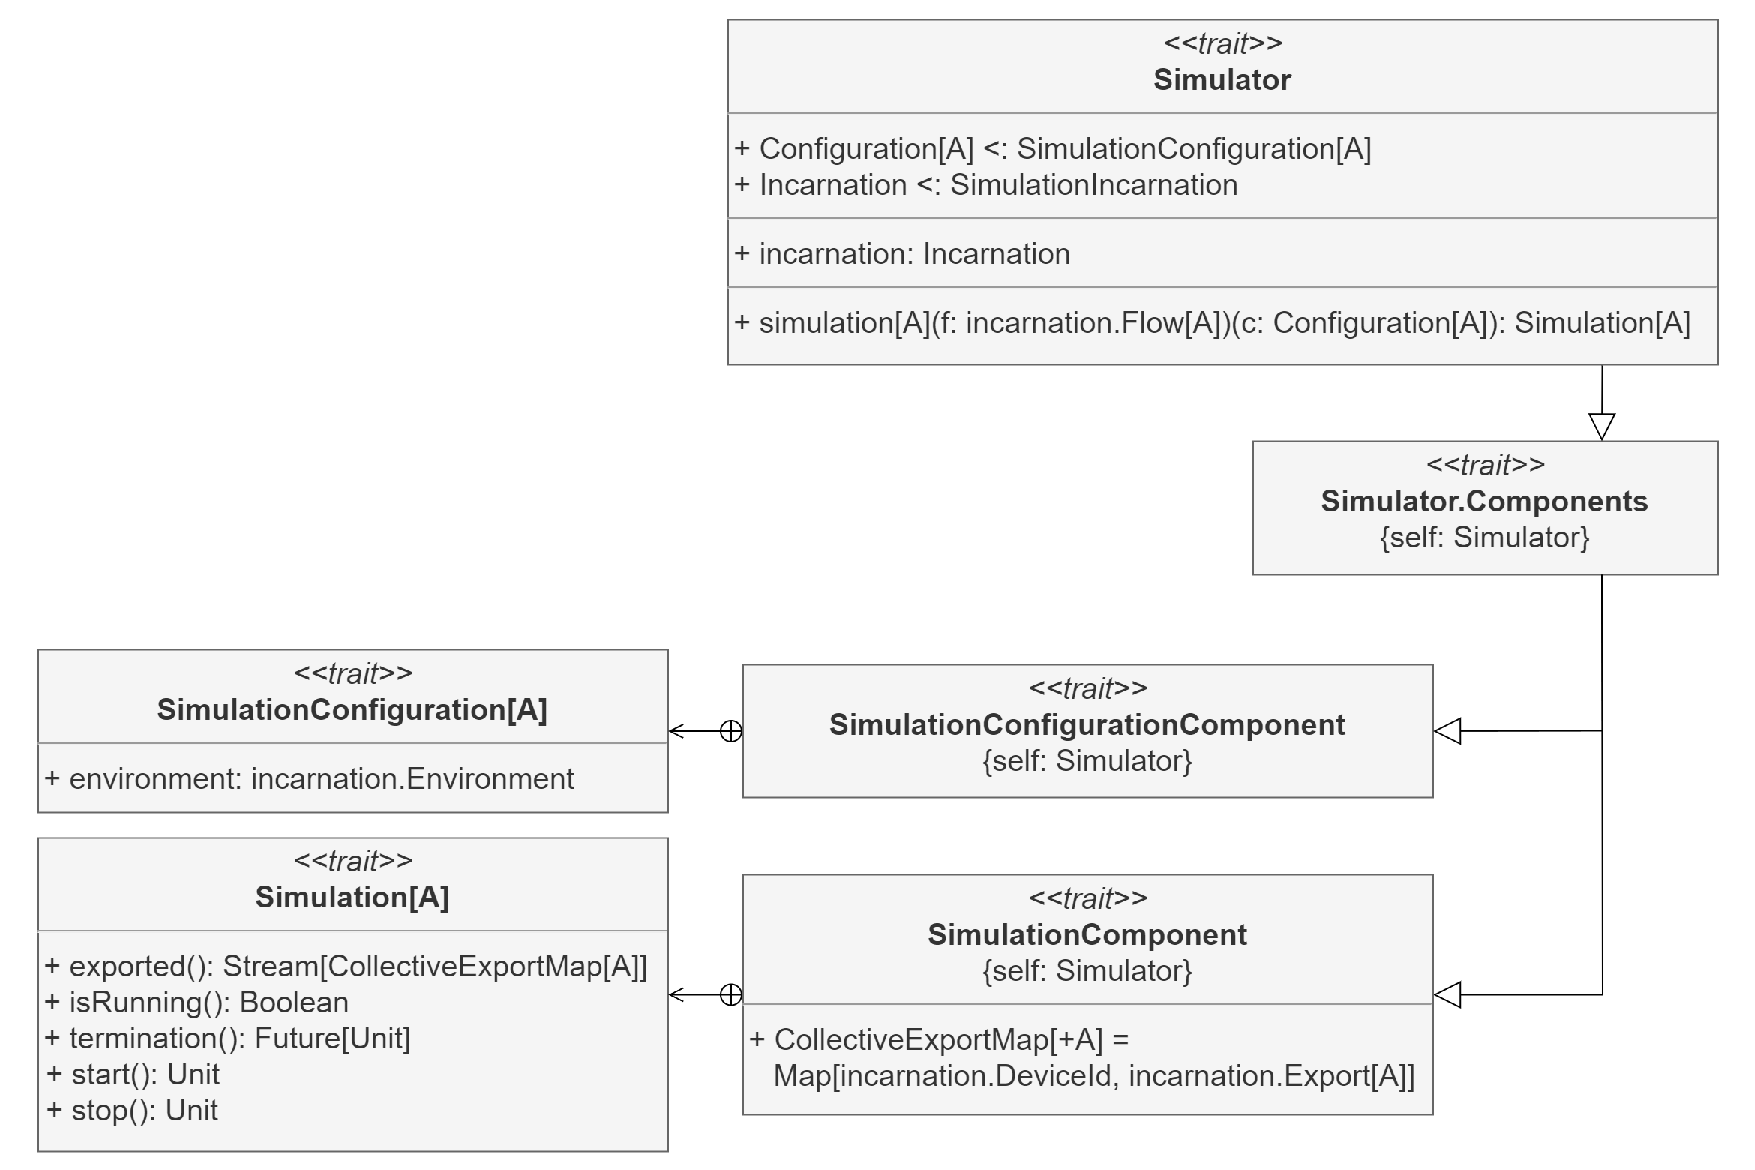
\includegraphics[width=1\textwidth]{resources/figures/diagrams/short/simulator-class-diagram.pdf}
  \caption[A UML class diagram of the simulator]{
    A UML class diagram of the simulator and its components.
  }
  \label{figure:simulator-class-diagram}
\end{figure}

A \texttt{Simulator} can be used to create several \texttt{Simulation}s, each
one requiring a \texttt{Flow}, that is a FRASP specification, and a
\texttt{Configuration}, which includes the \texttt{Environment} where the
aggregate is situated. To define the concepts of \texttt{Flow} and
\texttt{Environment}, a \texttt{Simulator} relies on a specific
\texttt{SimulationIncarnation}, which is an instance of the aggregate computing
\ac{DSL} in FRASP, tailored for simulation.

The implementation of the \texttt{Simulator} follows the \textit{cake pattern},
in which dependencies are defined inside external mixin components and can be
imported by extending the desired components. In particular, \texttt{Simulator}
depends on the \texttt{Simula\-tionConfigurationComponent}, which defines the
concept of \texttt{SimulationConfi\-guration}, and the
\texttt{SimulationCompo\-nent}, which defines the concept of
\texttt{Simula\-tion}. In the following sections, specializations of
\texttt{Simulator} defines additional concepts using other components, adhering
to the same naming convention.

As per design, a \texttt{Simulation} provides observability by means of the
methods \texttt{exported}, which supplies a \texttt{Stream} of all the device
exports transmitted within the aggregate, \texttt{exportedBy}, which supplies a
\texttt{Stream} of all the exports of a single device (\textit{an individual
view}), and \texttt{exportedByAll}, which supplies a \texttt{Stream} of all the
device exports accumulated during the simulation (\textit{a global view}, in
which each event is a \texttt{CollectiveExportMap}, that is a map from the
devices to their latest export). Similar methods are provided to observe only
the result of the computations, that is the root of the device exports.

Concerning controllability, a \texttt{Simulation} exposes one method
\texttt{start} to begin its execution, running the underlying
\texttt{startBehavior} of the concrete type of \texttt{Simulation}, and another
method \texttt{stop} to halt it, running the underlying \texttt{stopBehavior}
likewise. Moreover, a method \texttt{isRunning} can be used to know if the
simulation has already started but has not stopped yet, while another method
\texttt{termination} allows reacting to the end of the simulation.

% ! TeX root = ../../master-thesis.tex

\section{Step Simulator}
\label{section:implementation:step-simulator}

The implementation of a step simulator is represented by the class diagram in
Figure \ref{figure:step-simulator-class-diagram}, which is based on the design
described in Section \ref{section:design:step-simulation}.

\begin{figure}[!ht]
  \centering
  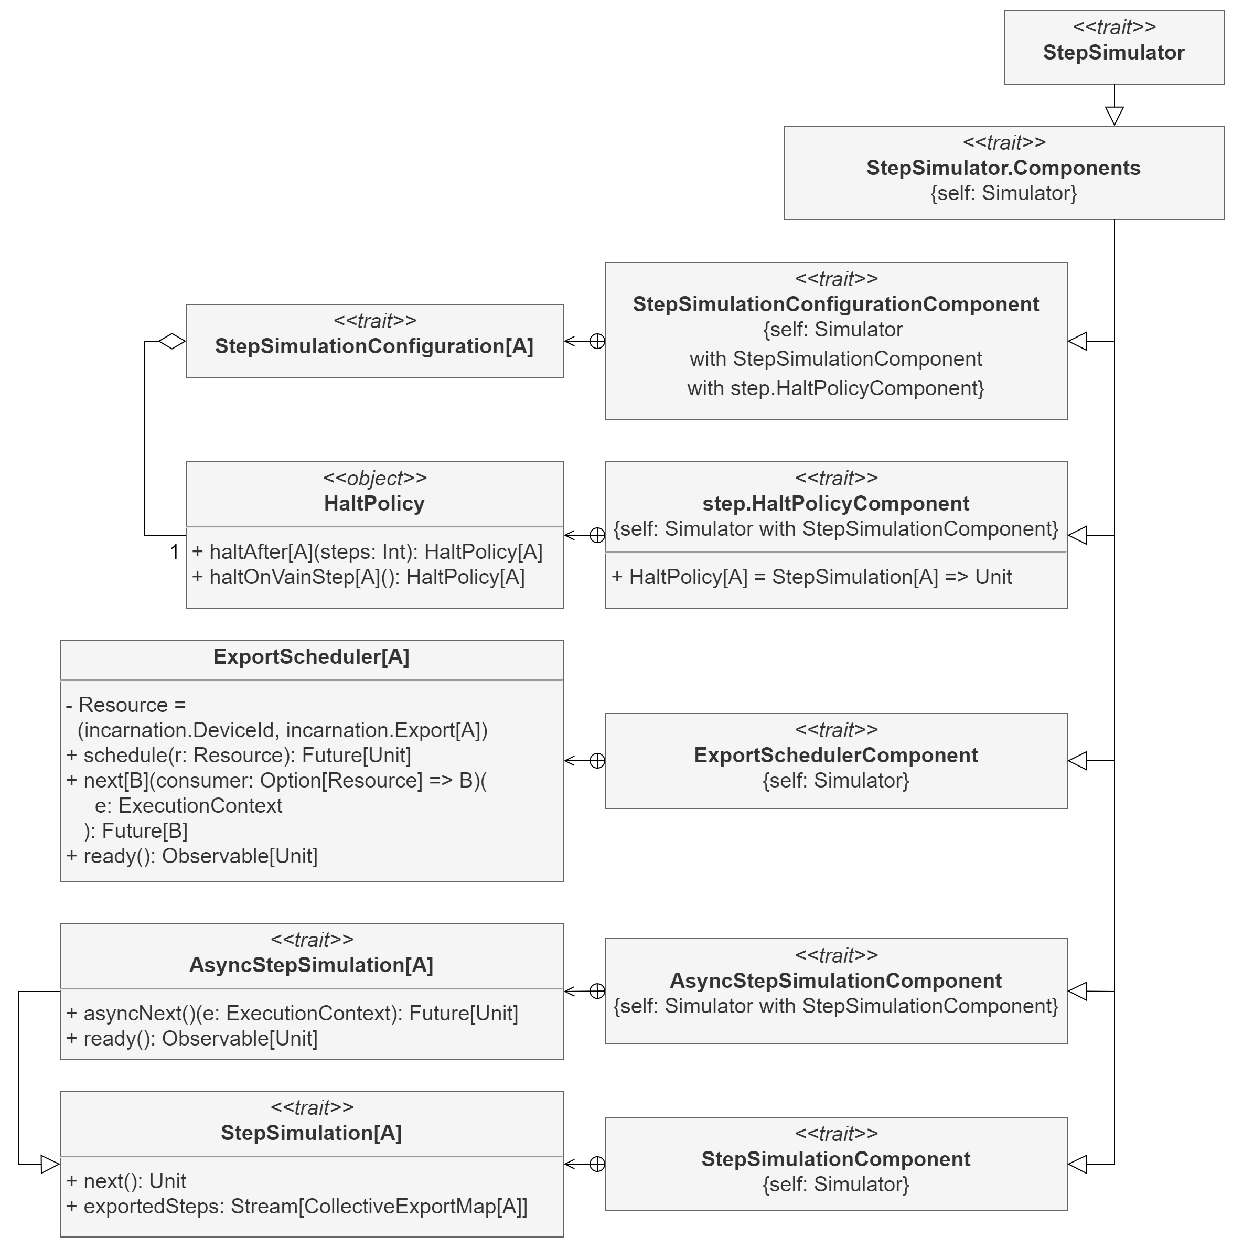
\includegraphics[width=1\textwidth]{resources/figures/diagrams/short/step-simulator-class-diagram.pdf}
  \caption[A UML class diagram of the step simulator]{
    A UML class diagram of the step simulator and its components.
  }
  \label{figure:step-simulator-class-diagram}
\end{figure}

A \texttt{StepSimulator} is a \texttt{Simulator} that creates
\texttt{StepSimulation}s. As per design, a \texttt{StepSimulation} provides
enhanced observability and controllability by means of the methods
\texttt{next}, which executes a step of the simulation by transmitting the next
device export to the neighbors and the user, and \texttt{exportedSteps}, which
supplies a \texttt{Stream} of the device exports transmitted at each step.

A thread-safe variant of \texttt{StepSimulation} is the
\texttt{AsyncStepSimulation}, which provides a new method \texttt{asyncNext},
executing the next step of the simulation in a given \texttt{ExecutionContext},
and a new property \texttt{ready}, allowing registering callbacks to execute
each time a new export is available for transmission. Actually, only an
implementation of \texttt{AsyncStepSimulation} has been developed at the
moment, meaning that every \texttt{StepSimulation} is an
\texttt{AsyncStepSimulation} under the hood. In the future, a specific
implementation of \texttt{StepSimulation} may be developed to be optimized for
single-threaded execution.

Specifically, the implemented \texttt{AsyncStepSimulation} involves keeping
track of the device exports through per-device queues, deferring their
transmission to the neighbors until requested by the user, that is when the
methods \texttt{next} or \texttt{asyncNext} are called, which delegate the
propagation of change to the user or to an \texttt{ExecutionContext}
respectively. The device queues are managed by an \texttt{ExportScheduler}:
each time an export is produced, the method \texttt{schedule} of the scheduler
is called, queuing the device export for later consumption; each time the next
step of the simulation is requested by the user, the method \texttt{next} of
the scheduler is called, dequeuing and transmitting the next export both to the
neighbors and the user. The transmission to the user happens by pushing the
exports into the \texttt{exportedSteps} stream. If all the device queues are
empty, an empty event is pushed instead.

The \texttt{ExportScheduler} decides the order of transmission of the device
exports, preserving the order of computation for each device (i.e., the export
of a device cannot be transmitted before its previous export). In particular,
the scheduling policy adopted by the current implementation is a best-effort
round-robin, in which each device is given the same chance to transmit its
exports as long as they have some to transmit, guaranteeing fairness during the
simulation.

The \texttt{SimulationConfiguration} of a \texttt{StepSimulation} is modeled by
the class \texttt{StepSimulationConfiguration}. In addition to the
\texttt{Environment}, the configuration includes an \texttt{HaltPolicy}, which
contains the logic for determining the end of the simulation. Some built-in
\texttt{HaltPolicy}s are already defined in the corresponding simulator
component, namely: \texttt{never}, which never halts the simulation (the user
may still stop it at any time); \texttt{haltWhen}, which halts the simulation
when a given predicate holds for the state of the aggregate;
\texttt{halt\-After}, which halts the simulation after a given number of steps;
finally, \texttt{haltOnVainStep}, which halts the simulation when a step is
executed, but all the export queues are empty. Additionally,
\texttt{HaltPolicy}s may be merged by means of the \texttt{combine} operator to
consider multiple conditions of termination, halting the simulation when any of
them is satisfied.

The \texttt{StepSimulationConfiguration} is interpreted by the
\texttt{StepSimulation} when the \texttt{start} method is called, creating the
devices of the aggregate, building its computational graph, scheduling the
first exports and setting up the \texttt{HaltPolicy}.

\paragraph{Example.}
A practical application of the \texttt{StepSimulator} is demonstrated in the
following program (Listing \ref{listing:step-simulator-example}).

\lstinputlisting[
  language=Scala,
  caption={
      [An application of the step simulator]
      An application of \texttt{StepSimulator}. The simulator is used to
      display the device exports on the standard output.
    },
  captionpos=b,
  label={listing:step-simulator-example}
]{resources/listings/step-simulator-example.txt}

% ! TeX root = ../../master-thesis.tex

\section{Concurrent Simulator}
\label{section:implementation:concurrent-simulator}

The implementation of a concurrent simulator is shown in the following class
diagram (Figure \ref{figure:concurrent-simulator-class-diagram}).

\begin{figure}[!ht]
  \centering
  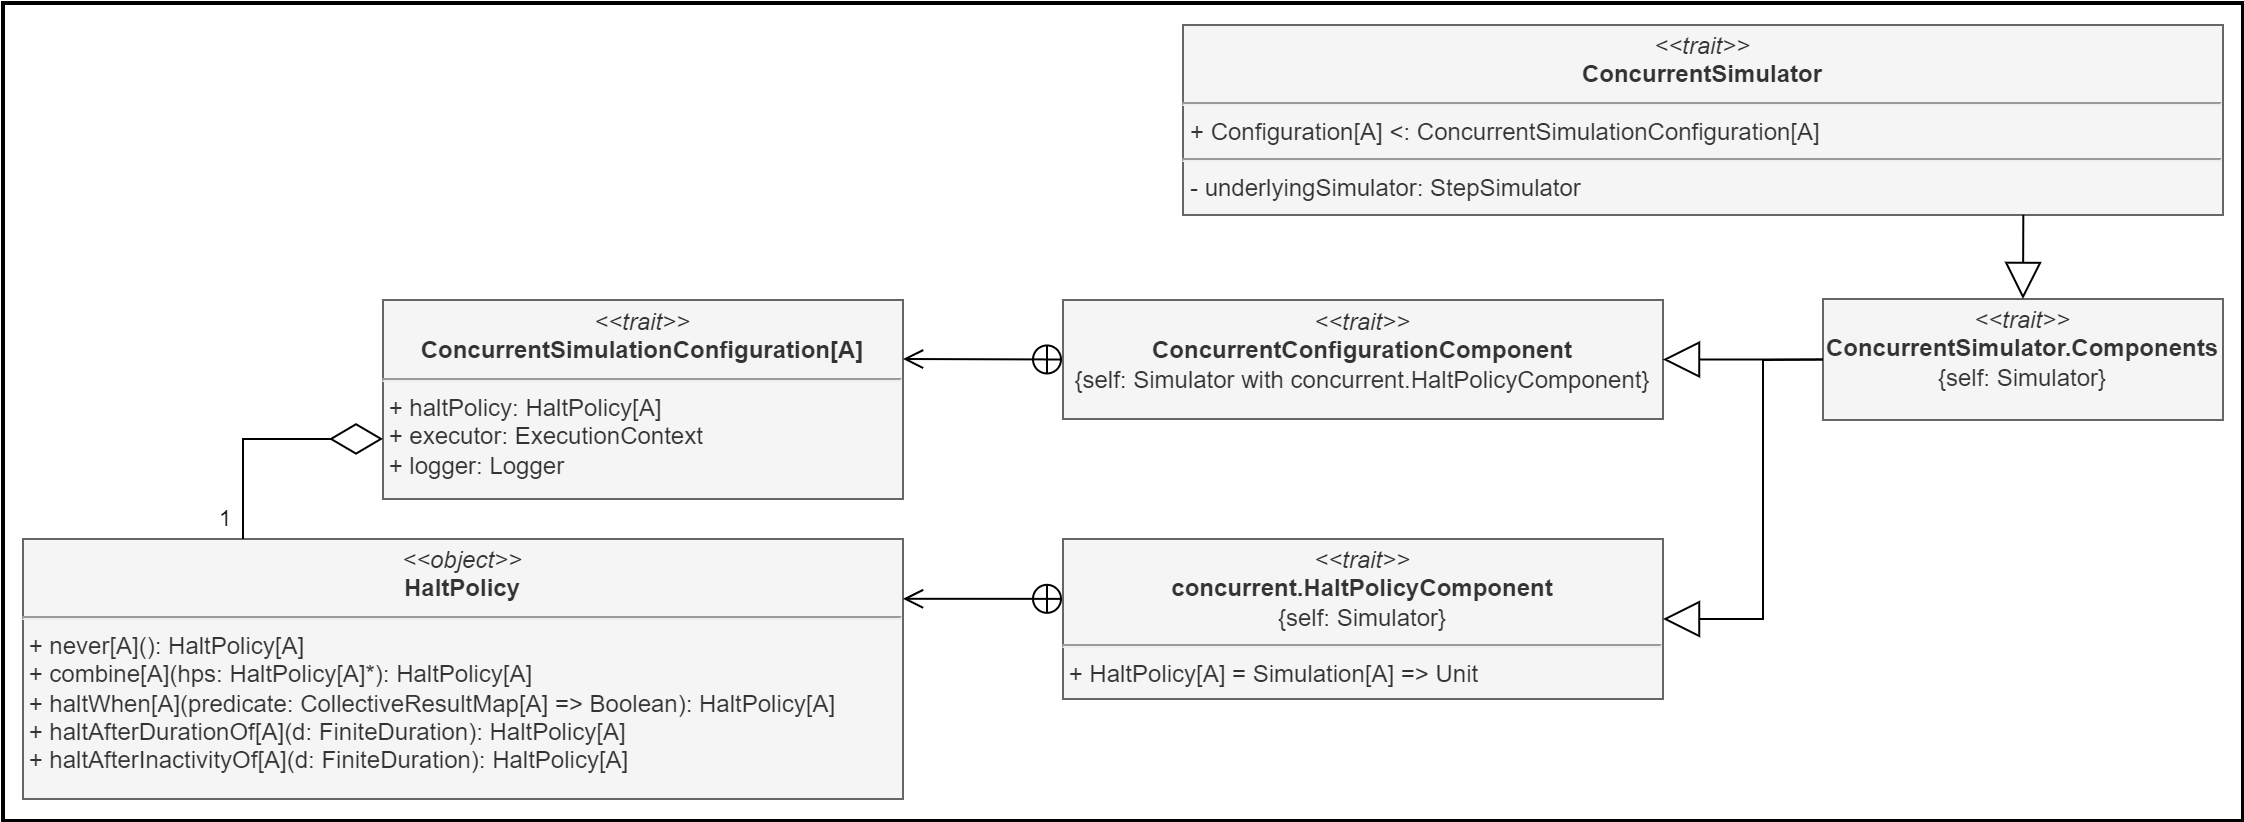
\includegraphics[width=1\textwidth]{resources/figures/concurrent-simulator-class-diagram.png}
  \caption[A UML class diagram of the concurrent simulator]{
    A UML class diagram of the concurrent simulator and its components.}
  \label{figure:concurrent-simulator-class-diagram}
\end{figure}

A \texttt{ConcurrentSimulator} is simply a \texttt{Simulator} whose
\texttt{Simulation}s are executed concurrently. A basic implementation of a
concurrent \texttt{Simulation} can be developed by leveraging an underlying
\texttt{AsyncStepSimulation}. In detail, the transmission of the device exports
to the neighbors and the user is delegated to an \texttt{ExecutionContext},
which schedules the computation on a thread pool. Transmission is scheduled as
soon as an export is generated, that is whenever the underlying simulation is
\texttt{ready}. As a consequence, from the perspective of the user, the
concurrent simulation behaves exactly the same as the base reactive model of
FRASP, without the increased observability of the step simulation, which would
have required further research to be developed due to the inherent challenges
of concurrency. Such development has been postponed since the concurrency of
the simulation did not translate to parallelism due to Sodium's transactions,
as better discussed in Section \ref{section:design:concurrent-simulation} of
the design.

The \texttt{SimulationConfiguration} of a concurrent \texttt{Simulation} is
modelled by the class \texttt{ConcurrentSimulationConfiguration}. In addition
to the \texttt{Environment} and \texttt{HaltPolicy}, the configuration includes
the \texttt{ExecutionContext} where the simulation will be executed. Some
built-in \texttt{HaltPolicy}s are already defined in the corresponding
simulator component, including \texttt{never}, \texttt{haltWhen} and two
others, namely \texttt{haltAfterDurationOf}, which halts the simulation after a
certain period of time has elapsed since its start, and
\texttt{haltAfterInactivityOf}, which halts the simulation after a certain
period of time has elapsed since its latest event.

\paragraph{Example.}
A practical application of the \texttt{ConcurrentSimulator} is demonstrated in
the following program (Listing \ref{listing:concurrent-simulator-example}).

\lstinputlisting[
  language=Scala,
  caption={
      [An application of the concurrent simulator]
      An application of \texttt{ConcurrentSimulator}. The program is very
      similar to Listing \ref{listing:step-simulator-example}, however, note
      that the concurrent simulator accepts a different configuration (line 10).
      Additionally, the exports are generated continually by the provided
      \texttt{ExecutionContext} after the simulation is started (after line 23,
      there is no \texttt{next} method to call).},
  captionpos=b,
  label={listing:concurrent-simulator-example}
]{resources/listings/concurrent-simulator-example.txt}

% ! TeX root = ../../master-thesis.tex

\section{Convergence Simulator}
\label{section:implementation:convergence-simulator}

The implementation of a convergence simulator is described by the class diagram
illustrated in Figure \ref{figure:convergence-simulator-class-diagram}.

\begin{figure}[!ht]
  \centering
  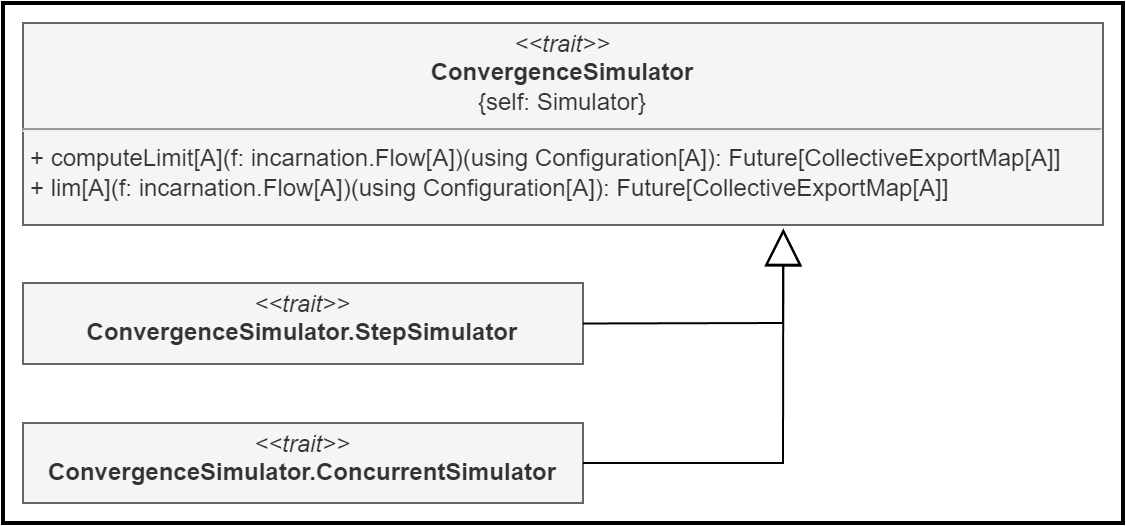
\includegraphics[width=0.60\textwidth]{resources/figures/convergence-simulator-class-diagram.png}
  \caption[A UML class diagram of the convergence simulator]{
    A UML class diagram of the convergence simulator
    and its concrete types.
  }
  \label{figure:convergence-simulator-class-diagram}
\end{figure}

A \texttt{ConvergenceSimulator} is a \texttt{Simulator} with the additional
ability of evaluating the stable state of an aggregate in self-stabilizing
specifications, namely the method \texttt{computeLimit} (or its shorthand
\texttt{lim}). The idea behind \texttt{computeLimit} is as simple as executing
a simulation until its termination, returning the last export transmitted by
each device in the network, in the form of a \texttt{CollectiveExportMap}.
Observation of the environment is possible by leveraging the device sensors
within the specification, attaching their percepts to the device exports.
However, to ensure that the result of \texttt{computeLimit} is a stable state
of the aggregate, the specification should be self-stabilizing and the
simulation should be halted after the aggregate has stabilized. Additionally,
if the aggregate has multiple possible non-deterministic stable states,
\texttt{computeLimit} can only evaluate one of them. Indeed, it may be useful
to consider only the root of the device exports to reduce the number of stable
states of the aggregate, possibly to a single deterministic stable state.

Given a self-stabilizing specification, the result of \texttt{computeLimit} is
determined by the \texttt{HaltPolicy} in the configuration specified by the
user. Below follows an analysis of the suitable \texttt{HaltPolicy}s and their
effects, assuming the user has complete control over the environment:
\begin{itemize}
  \item \texttt{haltWhen(\_ == $N_s$)}: calling $N_s$ the \textit{known} stable
        state of the aggregate, the simulation can be halted when the aggregate
        is in state $N_s$. This policy works for all simulations, however, it
        can only be used for evaluating the \textbf{reachability} of the state
        $N_s$ (\enquote{sometimes $N_s$ holds}), which is a looser property
        compared to convergence (\enquote{sometimes $N_s$ holds forever}).
  \item \texttt{haltAfterDurationOf(T)}: if a stable state exists, after an
        infinite amount of time the aggregate will have certainly stabilized.
        In general, the longer a simulation is executed (i.e., $T$), the
        higher the chances of the aggregate having stabilized. This policy
        works for all simulations, however, relying on real-world time
        introduces non-deterministic results.
  \item \texttt{haltAfterInactivityOf(T)}: inactivity in the simulation can be
        interpreted as a symptom of stability in the aggregate. In general,
        the longer the simulation is inactive (i.e., $T$), the higher the
        chances of the aggregate having stabilized. This policy works the same
        as \texttt{haltAfterDurationOf}, albeit possibly being more flexible
        (e.g., the same value of $T$ may apply to a larger variety of
        simulations).
  \item \texttt{haltAfter(N)}: similar to \texttt{haltAfterDurationOf}, but it
        relies on the steps of a simulation in order to track the simulation
        time. This policy offers deterministic results for deterministic
        simulations, however, it can only be used for \texttt{StepSimulation}s.
  \item \texttt{haltOnVainStep}: this policy guarantees to halt the simulation
        when the aggregate has stabilized, however, it can only be used for
        \texttt{StepSimulation}s.
\end{itemize}

At the moment, two concrete implementations of \texttt{ConvergenceSimulator}
are available, based on the \texttt{StepSimulator} and
\texttt{ConcurrentSimulator}.

\paragraph{Example.}
A practical application of the \texttt{ConvergenceSimulator} is demonstrat\-ed
in the following program (Listing \ref{listing:convergence-simulator-example}).

\lstinputlisting[
  language=Scala,
  caption={
      [An application of the convergence simulator]
      An application of \texttt{ConvergenceSimulator}. The program
      evaluates the stable states for three similar specifications
      (lines 21-23), in which each device counts all the integer numbers in a
      given range. For simplicity, the stable states only show the root of the
      devices exports.
    },
  captionpos=b,
  label={listing:convergence-simulator-example}
]{resources/listings/convergence-simulator-example.txt}

% ! TeX root = ../../master-thesis.tex

\section{Stream Extension}
\label{section:implementation:stream-extension}

In support of the simulators and the test suite, the set of operations on
\texttt{Stream}s provided by Sodium has been extended with new operators for
the manipulation, analysis, and monitoring of \texttt{Stream}s. In designing
these operators, care was taken to preserve compositionality, implementing them
as pure functions, and fluency, integrating them into the existing
\texttt{Stream} class by means of Scala's \textit{extension methods}, also
because inheritance of the base types of \texttt{Sodium} is not allowed.

The collection of implemented extension methods is provided by the
\texttt{StreamEx\-tension} object, as illustrated in Figure
\ref{figure:stream-extension-class-diagram}.

\begin{figure}[!ht]
  \centering
  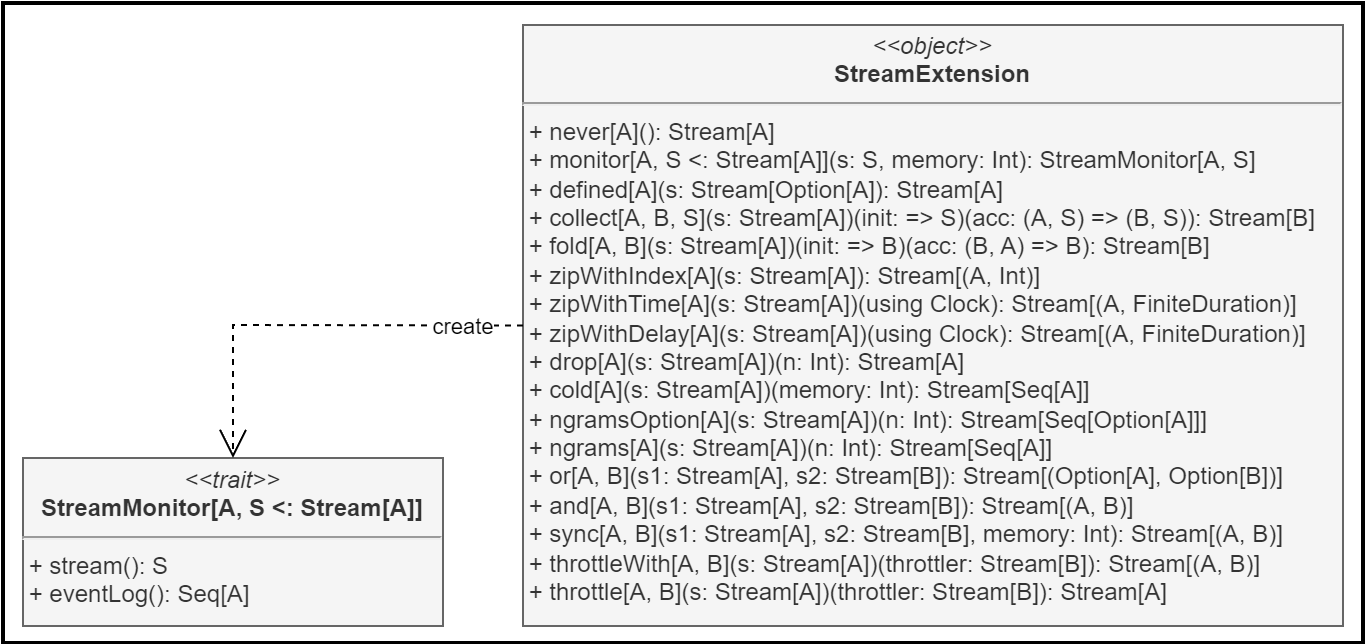
\includegraphics[width=0.8\textwidth]{resources/figures/stream-extension-class-diagram.png}
  \caption{
    A UML class diagram of the \texttt{Stream} extension
    and its operators.
  }
  \label{figure:stream-extension-class-diagram}
\end{figure}

\subsection{Persistence Operators}

The following operators can be used to deal with state persistence in
\texttt{Stream}s:

\begin{itemize}
  \item \texttt{collect}: evolve an initial state \texttt{init} as the
        input \texttt{Stream} $s$ generates new events and return an output
        \texttt{Stream} $s'$, whose events are a combination of the events
        fired by $s$ with the current state at the moment of firing. The
        \texttt{acc} function defines both the evolution of the state and the
        events of $s'$ depending on the firings of $s$.

        The \texttt{collect} operator is an adaptation for Scala of the
        homonymous operator provided by \texttt{Sodium} in Java.

  \item \texttt{fold}: a simplification of the \texttt{collect}
        operator, in which the events of the output \texttt{Stream} $s'$ are a
        snapshot of the current state taken at each firing of the input
        \texttt{Stream} $s$. The \texttt{acc} function defines the evolution of
        the state depending on the firings of $s$, and the events of $s'$ as a
        consequence.

        The \texttt{fold} operator is an implementation of the \textit{folding}
        operation provided by Scala for all \texttt{Iterable}s. However, the
        events of the input \texttt{Stream} are folded lazily as they are
        fired.
\end{itemize}

An example of their application is the evolution of the global view of an
aggregate, such as the method \texttt{exportedByAll}, obtained by accumulating
the individual device exports generated during a simulation.

\subsection{Temporal Operators}

The following operators can be used to perform time-sensitive analysis on
\texttt{Stream}s:

\begin{itemize}
  \item \texttt{zipWithIndex}: when applied to an input \texttt{Stream} $s$,
        return an output \texttt{Stream} $s'$, whose events are the same events
        of $s$ paired with the discrete time when they were fired. Discrete
        time is modelled as the number of firings preceding an event in $s$.
  \item \texttt{zipWithTime}: when applied to a \texttt{Stream} $s$, return an
        output \texttt{Stream} $s'$, whose events are the same events of $s$
        paired with the continuous time when they were fired. Continuous time
        is defined by a given \texttt{Clock}, which defaults to the number of
        nanoseconds elapsed since the creation of $s'$. Abstracting over
        real-world time allows the user to provide their own implementation of
        \texttt{Clock} to achieve complete control on the timeline of the
        \texttt{Stream}, which can be useful to avoid non-determinism during
        tests.
  \item \texttt{zipWithDelay}: when applied to an input \texttt{Stream} $s$,
        return an output \texttt{Stream} $s'$, whose events are the same events
        of $s$ paired with the continuous time elapsed since the previous
        event. Similarly to \texttt{zipWithTime}, continuous time is defined by
        a given \texttt{Clock}.
\end{itemize}

An example of their application is the implementation of time-sensitive
\texttt{Halt\-Policy}s, such as the \texttt{haltAfter} policy, introduced in
Section \ref{section:implementation:step-simulator}.

\subsection{Derivation Operators}

The following operators can be used to perform trend and behaviour analysis on
\texttt{Stream}s:

\begin{itemize}
  \item \texttt{ngrams}: when applied to an input \texttt{Stream} $s$, return
        an output \texttt{Stream} $s'$, whose events are all the possible
        groups of consecutive events fired by $s$ with cardinality $n$. Note
        that $s'$ does not fire any event until $s$ has emitted at least $n$
        events, which may never happen. In such case, any information about the
        events of $s$ is lost in $s'$.
  \item \texttt{ngramsOption}: as \texttt{ngrams}, but information loss is
        prevented by producing incomplete groups in $s'$ until $s$ has
        generated at least $n$ events. An incomplete group contains all the
        consecutive events fired by $s$ and as many placeholder values needed
        to reach cardinality $n$. In particular, \texttt{Option.None} is used
        as a placeholder value.
\end{itemize}

A future application of these operators could be the verification of more
sophisticated temporal properties against the evolution of aggregates, checking
the behaviour of the aggregate during a fixed time-window (e.g., evaluating if
the sum of the outputs of all the devices is always the sum at the previous
step plus one).

\subsection{Monitoring Operators}

The following operators can be used to monitor the events generated by
\texttt{Stream}s:
\begin{itemize}
  \item \texttt{cold}: when applied to an input \texttt{Stream} $s$, return an
        output \texttt{Stream} $s'$, whose events are sequences containing all
        the firings of $s$ after the creation of $s'$. Since $s$ may fire
        events indefinitely, the length of the sequences can be limited to a
        given amount of \texttt{memory}, which corresponds to the number of
        events of $s$ kept in memory by the operator. When the memory is full,
        the oldest events are replaced with the newest ones as they are fired.

        The name of this operator comes from the notion of \textbf{cold
        observable}s, as described in Section 6.2.1 of the book \cite{FRP}. In
        Sodium, all \texttt{Stream}s are inherently \textbf{hot observable}s,
        meaning that any dependent will react only to the events that are fired
        after its dependency has been declared, ignoring all the events that
        were fired before. The \texttt{cold} operator creates a \texttt{Stream}
        that acts \textit{almost} as a cold observable variant of the original
        \texttt{Stream}, by letting the dependents react also to the events
        that were fired before the declaration of their dependencies. However,
        dependents will be notified of all the events of the original
        \texttt{Stream} only after its next firing, which may never happen. To
        solve this problem, the \texttt{Stream} can be transformed into a
        \texttt{Cell} by means of the \texttt{hold} operator, obtaining an
        actual cold observable. In fact, \texttt{Cell}s propagate their latest
        state as soon as a dependent is declared.

  \item \texttt{monitor}: when applied to an input \texttt{Stream} $s$, return
        a \texttt{StreamMonitor} wrapping $s$. A \texttt{StreamMonitor} relies
        on the \texttt{cold} operator to monitor the wrapped \texttt{Stream},
        exposing a sequence of all its events, accessible at any time by means
        of the method \texttt{eventLog}. In other words, a
        \texttt{StreamMonitor} converts a \texttt{Stream} into an up-to-date
        list of its events. Similarly to the \texttt{cold} operator, the length
        of the sequence can be limited to reduce memory costs.
\end{itemize}

The purpose of these operators is to decouple the generation of the events of a
\texttt{Stream} from the evaluation of their properties, which greatly
simplifies testing. However, performing the evaluation during the generation of
the events would be more efficient, as the program generating the events could
be interrupted prematurely if the property was already proven before the
program termination. Naturally, this optimization cannot be implemented by
leveraging these operators, since the evaluation starts only after the program
termination.

An example of their application is the implementation of most of the test suite
and the \texttt{ConvergenceSim\-ulator}, in which the global view of the
aggregate is monitored to return its latest state when the simulation is
halted.

\subsection{Throttling Operators}

The following operators can be used to control the throughput of
\texttt{Stream}s:
\begin{itemize}
  \item \texttt{sync}: combine two input \texttt{Stream}s $s_1$ and $s_2$,
        returning an output \texttt{Stream} $s'$, whose events are the pairs of
        corresponding events in $s_1$ and $s_2$. More formally, the $k^{th}$
        event of $s'$ is a pair containing the $k^{th}$ event of $s_1$ and the
        $k^{th}$ event of $s_2$. Since $s_1$ and $s_2$ may fire their $k^{th}$
        event at different times, the operator requires keeping in memory the
        latest unpaired events of both \texttt{Stream}s. Similarly to the
        \texttt{cold} and \texttt{monitor} operators, the number of events
        stored for each \texttt{Stream} can be limited to a given
        \texttt{memory}.

        An implication of the \texttt{sync} operator is that the throughput of
        the output \texttt{Stream} is equal to the lowest throughput between
        the input \texttt{Stream}s, meaning that the operator can be used to
        control the frequency at which a \texttt{Stream} emits its events.
        Additionally, by limiting the memory of the operator, some events of
        the \texttt{Stream} with the highest throughput may be discarded when
        the memory is full, preventing possible overloads of its dependents.
  \item \texttt{throttleWith}: a specialization of the \texttt{sync} operator
        with unitary \texttt{memory}, storing only the latest unpaired event of
        each input \texttt{Stream}.
  \item \texttt{throttle}: a specialization of the \texttt{throttleWith}
        operator, in which the output \texttt{Stream} $s'$ fires the events of
        the first input \texttt{Stream} $s_1$, while the second input
        \texttt{Stream} $s_2$ acts only as a throttle for $s_1$.
\end{itemize}

A future application of these operators could be regulating the event
production rate of reactive variables in general, including \texttt{Stream}s,
\texttt{Cell}s and possibly \texttt{Flow}s.

% ! TeX root = ../../master-thesis.tex

\section{Finite Stream Extension}
\label{section:implementation:finite-stream-extension}

Another extension implemented for the Sodium library is the
\texttt{FiniteStreamExten\-sion}, which defines a new type of reactive variable
derived from \texttt{Stream}s, namely the \texttt{Finite\-Stream} type, as
illustrated in Figure \ref{figure:finite-stream-extension-class-diagram}.

\begin{figure}[!ht]
  \centering
  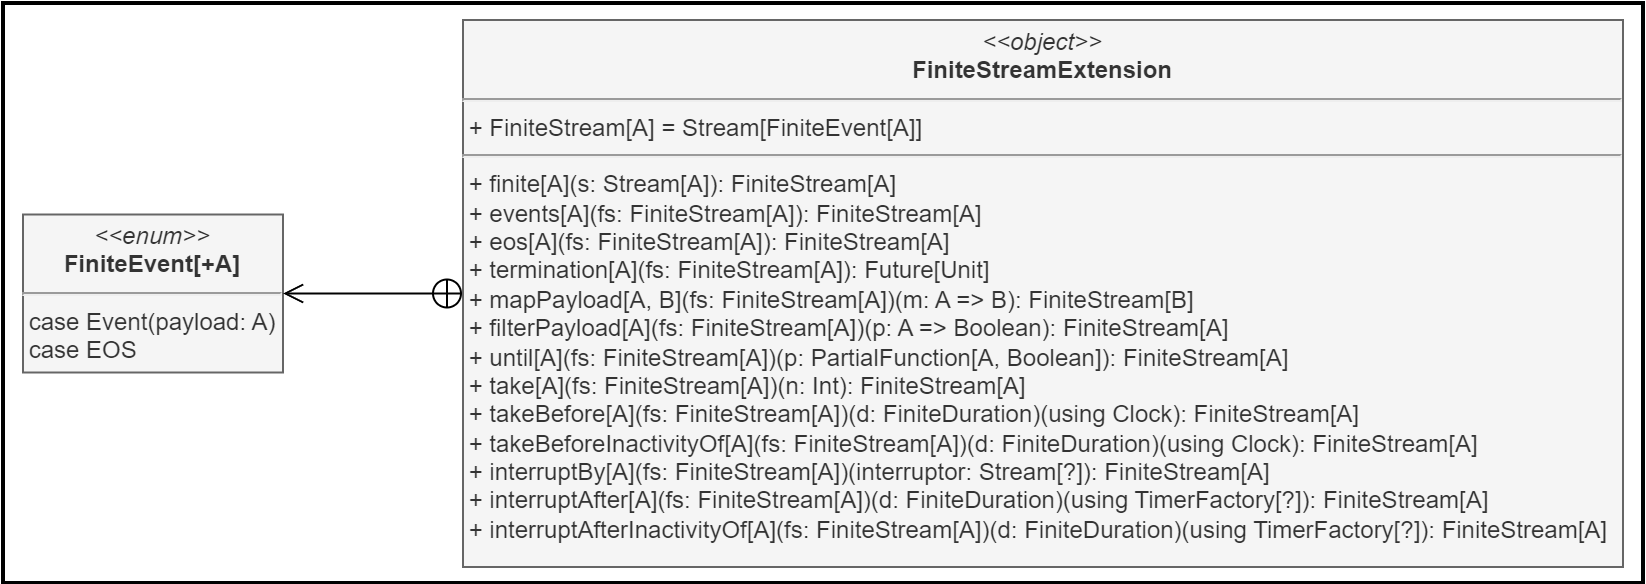
\includegraphics[width=1\textwidth]{resources/figures/finite-stream-extension-class-diagram.png}
  \caption[A UML class diagram of the finite stream extension]{
    A UML class diagram of the \texttt{FiniteStreamExtension}
    and its operators.
  }
  \label{figure:finite-stream-extension-class-diagram}
\end{figure}

In Sodium, \texttt{Stream}s may fire new events indefinitely, making them
suitable for modelling any type of producer. However, in their generality,
\texttt{Stream}s do not capture directly the fact that some producers only emit
a finite amount of events. For this purpose, \texttt{FiniteStream}s have been
designed to fire a finite amount of events before notifying all the dependents
of their termination.

Since extending \texttt{Stream}s is not allowed in Sodium,
\texttt{FiniteStream}s have been implemented as \texttt{Stream}s of
\texttt{FiniteEvent}s, which can either be \texttt{Event}s, wrapping a payload,
or an \texttt{EOS (End Of Stream)}, marking the termination of the stream. This
implementation allows leveraging the \texttt{Stream} operators also for
\texttt{FiniteStream}s, however, it does not restrict producers from emitting
additional events after the first \texttt{EOS}. To solve this problem, every
event following the first \texttt{EOS} is automatically discarded.

The \texttt{FiniteStreamExtension} provides a set of operators for creating
\texttt{Finite\-Stream}s, implemented in the form of Scala's extension methods,
similarly to the \texttt{StreamExten\-sion}. For better compositionality, these
operators have been designed to transform \texttt{FiniteStream}s into other
\texttt{FiniteStream}s. In fact, if the operators were transformations from
\texttt{Stream}s to \texttt{FiniteStream}s, they would wrap the firings of an
input \texttt{Stream} inside the \texttt{FiniteEvent}s of an output
\texttt{FiniteStream}. However, they could also be applied to
\texttt{FiniteStream}s, wrapping the \texttt{Finite\-Event}s of an input
\texttt{FiniteStream} inside the \texttt{FiniteEvent}s of an output
\texttt{Finite\-Stream}. As a consequence, any combination of operators would
create a \texttt{Stream} of nested \texttt{FiniteEvent}s, requiring recursive
unnesting to access the actual payload of the events. For this reason, the only
operator converting \texttt{Stream}s into \texttt{FiniteStream}s is the entry
point of the extension, namely the \texttt{finite} operator, which simply wraps
any event of an input \texttt{Stream} inside an \texttt{Event} of an output
\texttt{FiniteStream}.

The sole purpose of \texttt{finite} is to enable the application of the other
operators of the extension, namely:
\begin{itemize}
  \item \texttt{until}: when applied to an input \texttt{FiniteStream} $s$,
        return an output \texttt{Finite\-Stream} $s'$, obtained by halting $s$
        at the first event whose payload satisfies a given \texttt{predicate}.
  \item \texttt{take}: when applied to an input \texttt{FiniteStream} $s$,
        return an output \texttt{Finite\-Stream} $s'$, obtained by halting $s$
        after a given number of events.
  \item \texttt{interruptBy}: when applied to an input \texttt{FiniteStream}
        $s$, return an output \texttt{FiniteStream} $s'$, obtained by halting
        $s$ at the first event of a given \texttt{interruptor} stream.
  \item \texttt{takeBefore}: when applied to an input \texttt{FiniteStream}
        $s$, return an output \texttt{FiniteStream} $s'$, obtained by halting
        $s$ at the first event fired after a given \texttt{duration} has
        elapsed since the creation of $s'$.
  \item \texttt{interruptAfter}: when applied to an input \texttt{FiniteStream}
        $s$, return an output \texttt{FiniteStream} $s'$, obtained by halting
        $s$ after a given \texttt{duration} has elapsed since the creation of
        $s'$. The operator relies on a \texttt{Timer} to generate a
        notification after a set amount of time.
  \item \texttt{takeBeforeInactivityOf}: when applied to an input
        \texttt{FiniteStream} $s$, return an output \texttt{FiniteStream} $s'$,
        obtained by halting $s$ at the first event fired after a given
        \texttt{duration} has elapsed since its latest event.
  \item \texttt{interruptAfterInactivityOf}: when applied to an input
        \texttt{FiniteStream} $s$, return an output \texttt{FiniteStream} $s'$,
        obtained by halting $s$ after a given \texttt{duration} has elapsed
        since its latest event. The operator relies on a \texttt{Timer},
        similarly to \texttt{interruptAfter}.
\end{itemize}

An example of application of the \texttt{FiniteStreamExtension} is the
implementation of several \texttt{HaltPolicy}s for simulations, including
\texttt{haltAfterDurationOf} and \texttt{haltAfterInactivityOf} for concurrent
simulations.

% ! TeX root = ../../master-thesis.tex

\section{Dynamic Environments}
\label{section:implementation:dynamic-environments}

In support of the test suite, specifically for tests concerning sensors, an
explicit model of dynamic environments has been implemented. In fact, FRASP
provided only an explicit model of static environments, while changes in the
environment were supported with ad-hoc mechanisms, involving direct
modification of the \texttt{SimulationIncarnation} used to define the
specifications.

A basic implementation of a dynamic environment is the
\texttt{EnvironmentWith\-Tags} (Figure \ref{figure:environment-class-diagram}),
which is an \texttt{Environment} where devices can be linked to specific bits
of information, called \textit{tags}. In particular, the methods \texttt{tag}
and \texttt{untag} allow attaching and detaching tags from a set of devices,
while the method \texttt{withTag} can be used to retrieve the time-varying set
of the devices linked to a specific tag.

\begin{figure}[!ht]
  \centering
  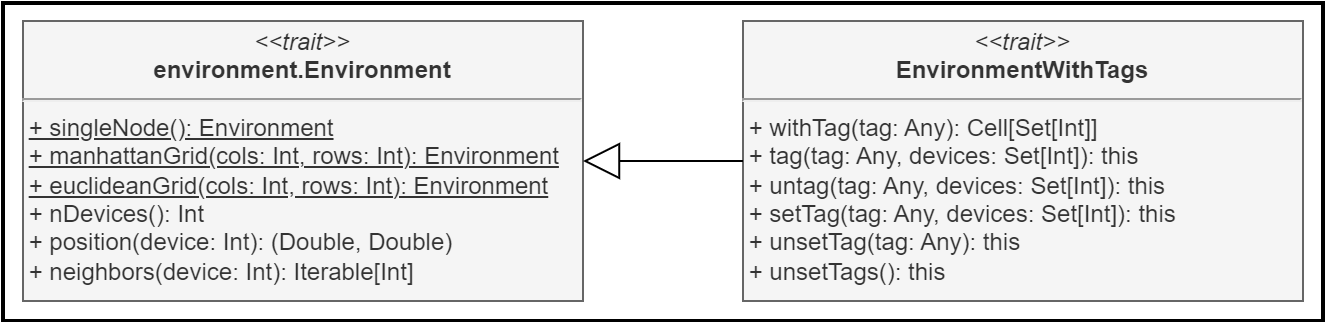
\includegraphics[width=0.8\textwidth]{resources/figures/environment-class-diagram.png}
  \caption{
    A UML class diagram of the environment types available
    for simulation.
  }
  \label{figure:environment-class-diagram}
\end{figure}

With the introduction of dynamic environments, the
\texttt{SimulationIncarnation} had to be updated to depend on an environment
type, instead of an environment instance (Figure
\ref{figure:simulation-incarnation-class-diagram}). Otherwise, the same
\texttt{SimulationIncarnation} could not be used to define different
specifications, as any program would be executed on the same environment,
already modified by previous programs, possibly causing unpredictable results.

\begin{figure}[!ht]
  \centering
  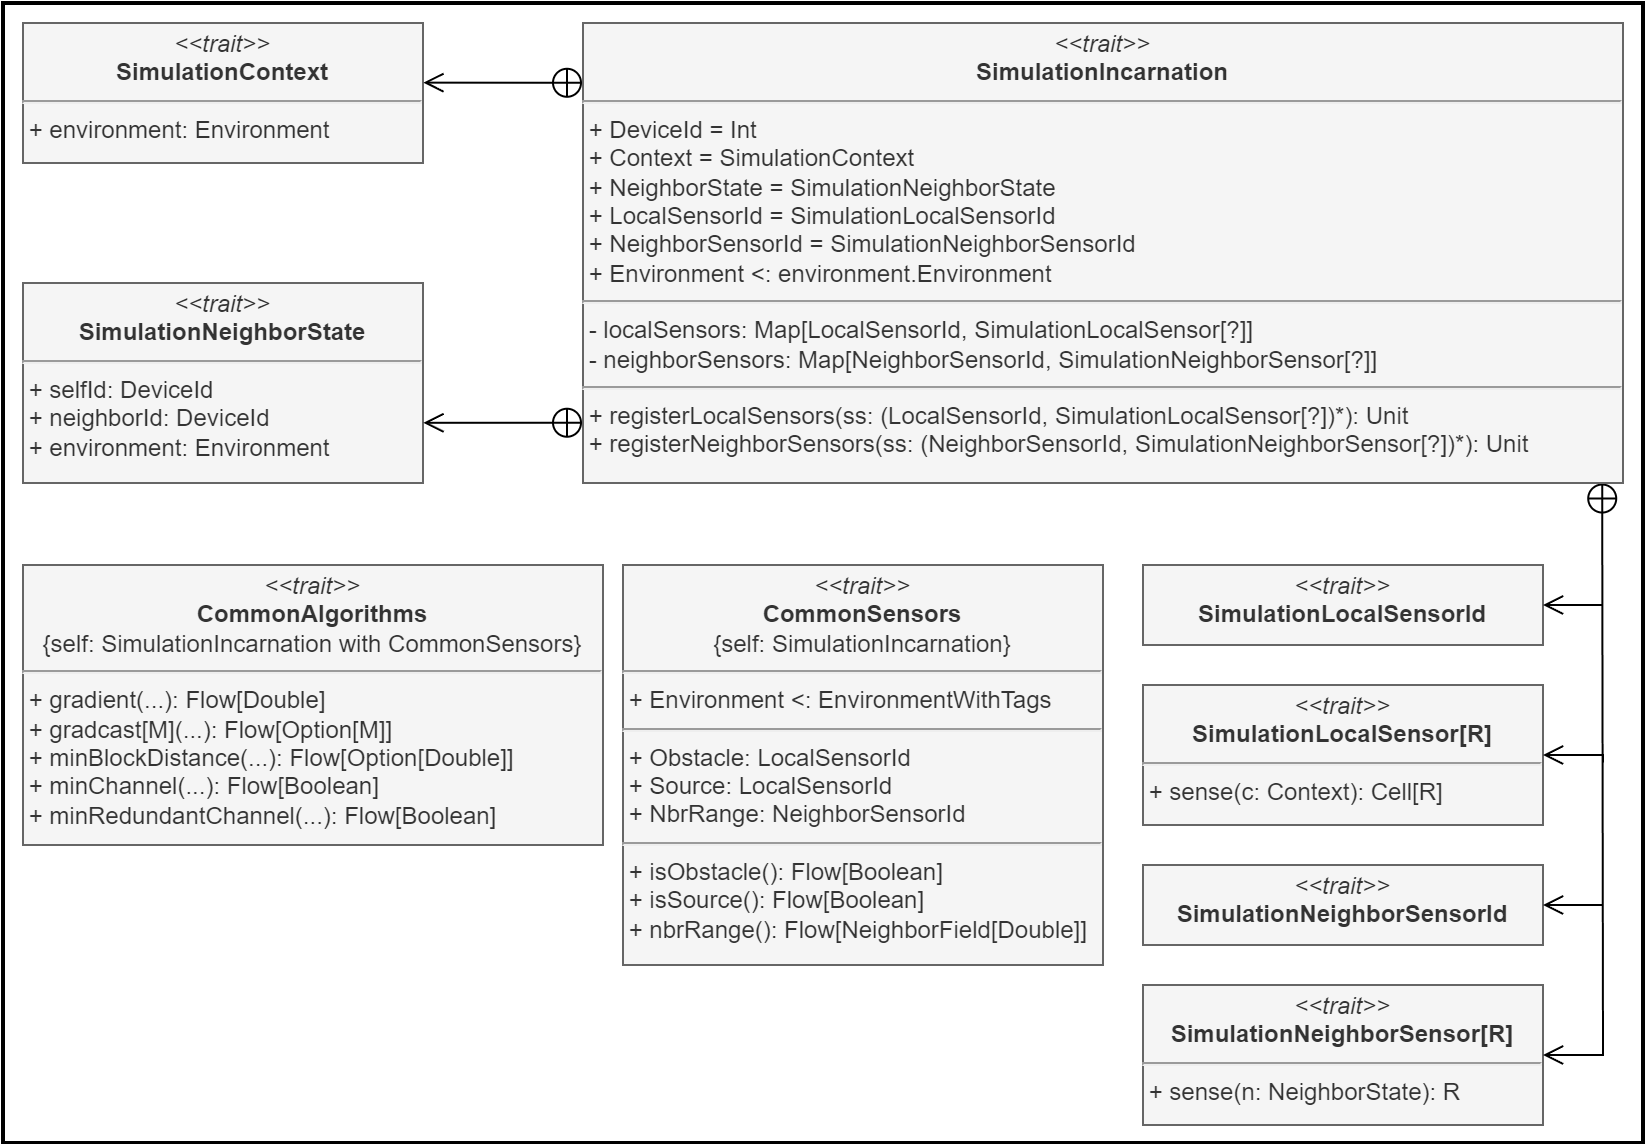
\includegraphics[width=0.85\textwidth]{resources/figures/simulation-incarnation-class-diagram.png}
  \caption{A UML class diagram of the new simulation incarnation.}
  \label{figure:simulation-incarnation-class-diagram}
\end{figure}

Additionally, the \texttt{SimulationIncarnation} has been improved to support
the registration of local and neighbour sensors, retrieving localized
information from the environment, instead of relying on information injected
directly into the \texttt{Simu\-lationIncarnation}. In detail, local sensors
are modelled by the trait \texttt{Simula\-tionLocalSensor}, which is a function
producing the readings of a given device in the environment. Local sensors can
be registered to the \texttt{SimulationIncar\-nation} under a specific
identifier, typed \texttt{SimulationLocalSensorId}, by which they can be
referenced using the \texttt{sensor} construct within an aggregate
specification. In a similar fashion, neighbour sensors are implemented by the
traits \texttt{SimulationNeighbor\-Sensor} and
\texttt{Simulation\-NeighborSensorId}.

To enhance modularization and isolation of concerns, the implementation of the
sensors has been extracted from the \texttt{SimulationIncarnation} and
delegated to specific traits (Figure \ref{figure:sensor-class-diagram}). In
particular, sensors are modelled by the trait \texttt{Sensor}, which declares
the type of environment where the sensor can be employed, namely
\texttt{SuitableEnviron\-ment}. A \texttt{Sensor} can be either a
\texttt{LocalSensor}, creating the corresponding
\texttt{Simula\-tion\-LocalSensor} for suitable
\texttt{SimulationIncarnation}s, or a \texttt{NeighborSensor}, creating the
corresponding \texttt{SimulationNeighborSensor} for suitable
\texttt{Simulation\-Incarnation}s. A \texttt{SimulationIncarnation} is suitable
for a \texttt{Sensor} if the \texttt{Environ\-ment} of the incarnation is a
\texttt{SuitableEnvironment} for the sensor.

\begin{figure}[!ht]
  \centering
  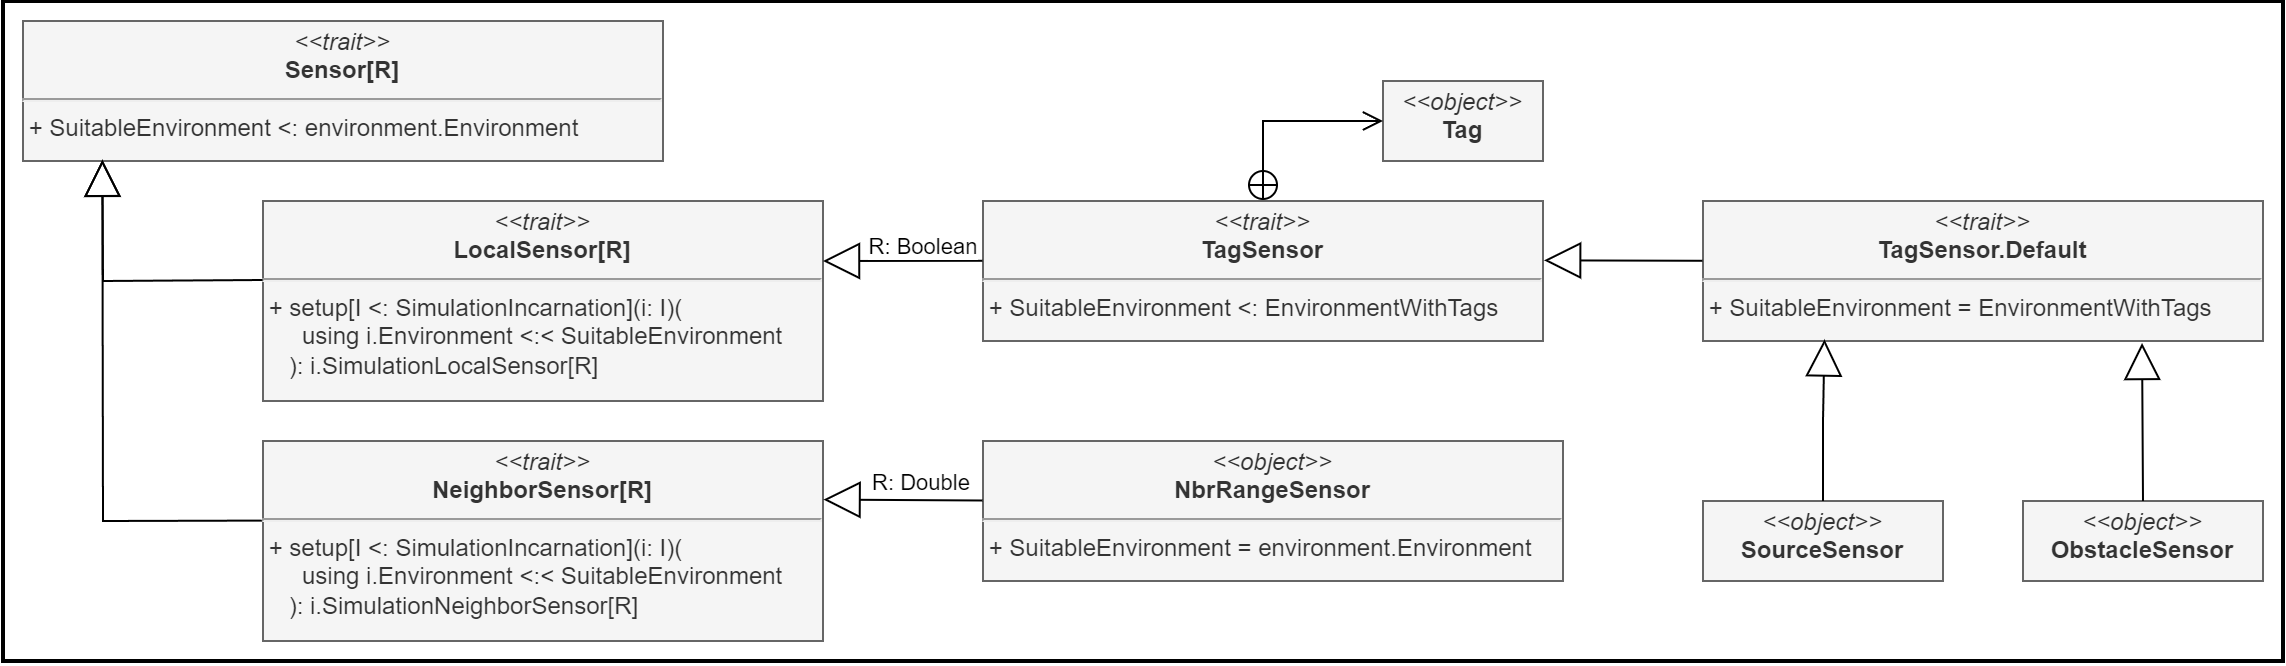
\includegraphics[width=1\textwidth]{resources/figures/sensor-class-diagram.png}
  \caption{A UML class diagram of the sensor types available for simulation.}
  \label{figure:sensor-class-diagram}
\end{figure}

Some built-in sensors have already been implemented, namely \texttt{TagSensor},
which is a \texttt{LocalSensor} detecting if a specific tag is linked to a
device (e.g., if the device is marked as an obstacle or a source), and
\texttt{NbrRangeSensor}, which is a \texttt{NeighborSensor} measuring the
distances from a device and all of its neighbours.

Finally, leveraging these concepts, two mixins for
\texttt{SimulationIncarnation}s have been implemented, namely the
\texttt{CommonSensors} mixin, extending the \ac{DSL} with a set of standard
sensors, and the \texttt{CommonAlgorithms} mixin, extending the \ac{DSL} with a
set of gradient-based algorithms.
